\chapter{Literature Review}
\label{ch:lit}

%TODO: Diagram - What issues do I cover, how are they linked? Soundscape practice, Acoustic Analysis, Predictive Modelling
%TODO: Content from Soundscape and the Built Environment, Chapter 10, Applied Soundscape Practice

\draft{Chapter Abstract}

\section{Introduction}

Traditional noise control methods face several challenges in decreasing noise pollution in modern cities. In many cases, these challenges stem from an approach primarily focussed strictly on decreasing the noise levels or noise exposure in a given space. Part of this approach stems from traditional assessment methods which centre the sound level as the sole metric and which struggle to account for additional sonic characteristics such as tonality or the meaning associated with a sound. In particular, the metrics used, particularly when attempting to adjust for these characteristics, are impractical to apply for complex sound environments\footnote{Throughout this thesis, I will use the phrase `complex sound environment' or `complex soundscape' to refer to a real-world environment with overlapping and competing sound sources which consist of sonic characteristics that any single metric currently struggles to encapsulate.} with several overlapping sound sources. This approach can often prove impractical in situations where a problematic noise source cannot be moved or decreased, or where mitigation methods such as building a sound wall to block the sound transmission are expensive, infeasible, or merely undesirable \cit{Ekici \& Hocine, 2003 (A Review of Research on Environmental Noise Barriers)}. This can result in many urban spaces which are intended to provide a restorative space in the city being unpleasant due to the unwanted noise and going underutilised with little way to address the issue. Where noise and acoustics is considered by planners and architects, their concern is typically with compliance of ordinances and regulations, or with maintaining the existing environmental conditions. Noise mitigation efforts frequently fail to centre human perception within the design \cit{Coelho ch. 8 in Kang and Schulte-Fortkampf, 2016}. 

\subsection{Noise assessment methods}
In this section I will begin with a review of some examples of noise assessment and mitigation methods. This will provide the existing context for how traditional noise control approaches are targeted. In the UK \citet{BS41422019} is the current reference document for assessing and addressing noise impacts in outdoor environments. In particular, BS 4142 is intended to assess the impact of a specific noise source when introduced to a given background level. BS 4142 makes use of a `rating level' based on a comparison between the sound which is being assessed and the background sound which would exist without it. Within the standard, a series of noise metrics are defined \citep[Sec. 3]{BS41422019}:

\begin{itemize}
  \item \textbf{ambient sound level, $L_a = L_{Aeq,T}$} - equivalent continuous A-weighted sound pressure level of the totally encompassing sound in a given situation at a given time, usually from many sources near and far, at the assessment location over a given time interval, \emph{T}.
  \item \textbf{background sound level, $L_{A90,T}$} - A-weighted sound pressure level that is exceeded by the residual sound at the assessment location for 90\% of a given time interval, \emph{T}, measured using time weighting, \emph{F}, and quoted to the nearest whole number of decibels.
  \item \textbf{equivalent continuous A-weighted sound pressure level, $L_{Aeq,T}$} - value of the A-weighted sound pressure level in decibels of continuous steady sound that, within a specificed time interval, $T = t_2 - t_1$, has the same mean-squared sound pressure as a sound that varies with time, and is given by the following equation:
    $$L_{Aeq,T} = 10 lg_{10} \left[\frac{1}{T} \int^{t_2}_{t_1} \frac{p_A(t)^2}{p_0^2}dt \right]$$
    where: \\
      \space $p_0$ is the reference sound pressure (20 $\mu Pa$); and\\
      \space $p_a{t}$ is the instantaneous A-weighted sound pressure (Pa) at time \emph{t}
  \item \textbf{residual sound level, $L_r=L_{Aeq,T}$} - equivalent continuous A-weighted sound pressure level of the residual sound\footnote{Ambient sound remaining at the assessment location when the specific sound source is suppressed to such a degree that it does not contribute to the ambient sound.} at the assessment location over a given time interval, \emph{T}.
  \item \textbf{specific sound level, $L_s=L_{Aeq,Tr}$} - equivalent continuous A-weighted sound pressure level produced by the specific sound source at the assessment location over a given reference time interval, $T_R$.
\end{itemize}

In each of these metrics, the primary sonic feature which is assessed is the sound level, with some consideration for frequency content by using A-weighting. The standard then sets out the procedure to be used to measure the existing background sound level, measure or estimate the level of the specific sound, and calculate the margin between the specific sound and the background sound level. Throughout this process, BS 4142 notes `certain acoustic features can increase the significance of impact over that expected from a basic comparison between the specific sound level and the background sound level.' To address this, it introduces certain methods to add a character correction to the specific sound level, resulting in the rating level:

\begin{itemize}
  \item \textbf{rating level, $L_{Ar,Tr}$} - specified sound level plus any adjustment for the characteristic features of the sound
\end{itemize}

The sonic characteristics included for these rating level adjustments are tonality, impulsivity, intermittency, and `other sound characteristics' (described as `otherwise readily distinctive against the residual acoustic environment'). As an example of how these adjustments are applied, I will quote the guidance to adjust for tonality \citep[pg. 13]{BS41422019}:

\begin{quote}
  \textbf{Tonality} \\
  For sound ranging from not tonal to prominently tonal the Joint Nordic Method \citep{ISO1996Part1} gives a correction of between 0 dB and + 6 dB for tonality. Subjectively, this can be converted to a penalty of 2 dB for a tone which is just perceptible at the noise receptor, 4 dB where it is clearly perceptivle, and 6 dB where it is highly perceptible.
\end{quote}

The goal of these rating level adjustments is to incorporate aspects of the specific perception of sound, which may make a sound more disturbing, more noticeable, or generally more impactful than the dBA value alone would suggest. This is an important part of rating the impact of these sounds and necessary to achieve the goals of the standard. However, by implementing this as adjustments in terms of dB, it still centres the sound level in the assessment and enables only a one-dimensional approach to assessing impact. 

While BS 4142 is targeted towards assessing the impact of a specific sound, and primarily in an industrial and commercial context, \citet{ISO1996Part1} is more general, including provisions for assessing `community noise'. In the Introduction to the standard, several acknowledgements are raised about the importance of human perception, but the primary focus on the sound level is confirmed:

\begin{quote}
  To be of practical use, any method of description, measurement, and assessment of environmental noise is intended to be related in some way to what is known about human response to noise. [\ldots] The methods and procedures described in this part of ISO 1996 are intended to applicable to noise from various sources, individually or in combination, which contribute to the total exposure at a site. At the stage of technology at the time of publication of this part of ISO 1996, the evaluation of long-term noise annoyance seems to be best met by adopting the adjusted A-weighted equivalent continuous sound pressure level, which is termed a ``rating level''. 
\end{quote}

Despite the nods toward a perception-focussed approach, ISO 1996 re-emphasises the focus on sound pressure level when it comes to discussing community noise annoyance\citep[Sec. 6.1]{ISO1996Part1}:

\begin{quote}
  If the sound has special characteristics, then the rating equivalent continuous sound pressure level shall be the primary measure used to describe the sound. [\dots] research has shown that different transportation sounds or industrial sounds evoke different community annoyance responses for the same A-weighted equivalent continuous sound pressure level.
\end{quote}

What this review of some of the relevant standards and guidance demonstrates is that the decibel (specifically the equivalent continuous sound pressure level) is the dominant rating metric for all types of environmental noise and that, despite attempts to incorporate adjustments for `special' characteristics of the sound, the only sonic characteristic really being considered is the sound level. In addition, what my review of this guidance reveals is that the rating level adjustments are impractical to apply to complex sound environments for general evaluation. \citet[Eq. 4]{ISO1996Part1} provides a formula for calculating the rating level of combined sources:

$$
L_{Req,T} = 10lg \left(\frac{1}{T} \sum_n \sum_j T_{nj} * 10^{0,1L_{Reqj,Tnj}}  \right) dB
$$

where

$$
T = \sum_n T_{nj}
$$

for each source \emph{j}.

However, ISO 1996 notes that `As a practical matter, Formula (4) is typically evaluated one source at a time.' This makes it clearly impractical as a method for assessing a general sound environment, with multiple competing sound sources, or for automated monitoring. In this way, these standards preclude the possibility of making use of the rating level to provide a more nuanced view of a sound environment which accounts for the sonic characteristics. This presents a particular challenge for considering how these sonic characteristics influence human perception in a noise mapping context. 

\subsection{Noise mapping and city-scale noise impacts}
The \gls{end} \citep{Directive200249ECEuropeanUniEuropean}, first implemented in 2002, is the main EU instrument to identify noise pollution impacts and track urban noise levels across the EU. Its goals were to determine the population's exposure to environmental noise, make information on environmental noise available to the public, and prevent and reduce environmental noise and its effects. \draft{cont.}

As can be seen in the structure and guidance of these standards documents, the goal is to maintain the existing sound environment and mitigate noise impacts from newly introduced sounds, with the dB, in terms of a rating level, as the metric of assessment. Attempts have been made across the various standards to include adjustments for how sonic characteristics such as tonality, impulsivity, and spectral content influence human perception in a useful and practical way. It should also be clear that, as expressed by Axelsson, these standards approach sound reactively, addressing it only as something to be managed, reduced, or tracked. Although the goals laid out in the \gls{end} have shown a shift to considering sound as a potential benefit to be protected and promoted, the assessment methods available are still rooted in the waste management approach. In the next section, I will review the evidence which suggests that, for the design of urban spaces, perception should be centred as the design and assessment goal and how the decibel fails to enable this.

\section{The importance of perception and experience}

\draft{From Ten Questions on Soundscape: Reducing sound levels, though, did not
necessarily lead to improved quality of life in urban and rural areas (e.g., Yang \&
Kang, 2005; Andringa, et al., 2013; van Kempen, Devilee, Swart, \& van Kamp, 2014;
Asdrubali, 2014; Alves, Estévez-Mauriz, Aletta, Echevarria-Sanchez, \& Puyana
Romero, 2015) and this is why the soundscape multidisciplinary approach to the
management of the acoustic environments became more and more relevant, for its
focus on how people actually perceive and experience the acoustic environments}

Despite being the dominant focus of urban noise mitigation, the reduction of sound levels has been proven to not necessarily correlate with perception or lead to improved health outcomes \citep{Kang2016Ten,Kang2006Urban} \cit{add the citations from above too}. Research from the early 2000s demonstrated that reducing the sound level does not necessarily lead to better acoustic comfort in urban areas \citep{DeRuiter2000Noise,SchulteFortkamp2001Quality}. \citet{Yang2005Acoustic} assessed the acoustic comfort of people in a 14 urban spaces of five European countries (Greece, Italy, UK, Germany, and Switzerland). For this study, users of the space were randomly selected in the spaces and asked to evaluate the subjective sound level on a scale from 1 (very quiet) to 5 (very noisy), while an additional measure of acoustic comfort was assessed (from 1 [very comfortable] to 5 [very uncomfortable]) in the 2 case study sites in Sheffield, UK. While each participant was interviewed, the researchers measured the 1-minute \gls{laeq} as well as additional microclimate indices. 

By examining the relationship between the sujective sound level and the measured sound level within each site separately, their results indicated an inconsistent relationship across sites, with correlation values ranging from $R=0.373$ for Sesto San Giovanni, Italy to $R=0.941$ for Karaisakaki square, Greece. This indicates that although \gls{lzeq} can be a good indicator for the subjective sound level, the strength of this relationship and in particular the slope of the relationship depends on other factors not captured by the dB(A). This is further reinforced by the acoustic comfort results. \cref{fig:yang2005acousticComfort} shows the acoustic comfort and sujective sound level ratings for the two Sheffield case study sites reported in \citet{Yang2005Acoustic}. Although in these sites there is a strong correlation between the \gls{laeq} and the subjective sound level, the correlation with acoustic comfort is much weaker. In addition, \cref{fig:yang2005acousticComfort}(b) in particular shows a nonlinear relationship between dB(A) and acoustic comfort. It can be seen that above \~70 dB(A) the acoustic comfort decreases as the sound level increases, however below 70 dB(A) there is no significant change in acoustic comfort. 

\begin{figure}
  \centering
  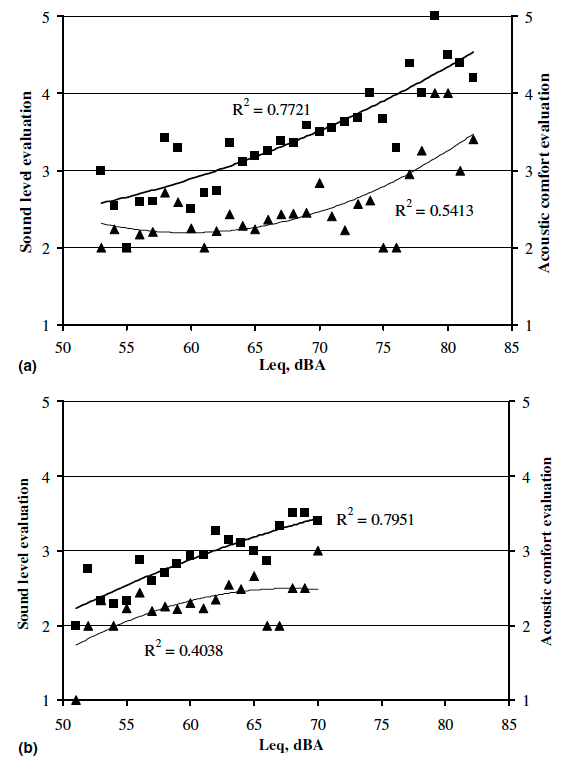
\includegraphics[width=.8\textwidth]{Figures/YangKang2005 Acoustic Comfort dB.png}
  \caption{Reproduced with permission from \citep[Fig. 2]{Yang2005Acoustic} showing subjective responses and measured sound levels in urban spaces in Sheffield, UK. Relationships between the measured sound level, the mean subjective evaluation of the sound level and the mean acoustic comfort evaluation, with binomial regressions and correlation coefficients squared $R^2$. (a) The Peace Gardens. (b) The Barkers Pool. $\blacksquare$ -- subjective evaluation of sound level (1 [very quiet]; 2 [quiet]; 3 [neither quiet nor noisy]; 4 [noisy]; 5 [very noisy]). $\blacktriangle$ -- acoustic comfort evaluation (1 [very comfortable]; 2 [comfortable]; 3 [neither comfortable nor uncomfortable]; 4 [uncomfortable]; 5 [very uncomfortable]). \label{fig:yang2005acousticComfort} }
\end{figure}



\paragraph{Parallels in visual perception}
\citet{Kruize2019Exploring} demonstrated that the experience and use of natural urban spaces were strongly related to health outcomes associated with those spaces, while strictly physical characteristics of the space were not. 
Their study made use of a cross-sectional design to investigate the relationships between several factors related to the experience of natural outdoor environments and key health outcome indicators. The outcome indicators investigated included physical activity, social contact, and mental health. As input indicators, they considered a set of GIS-derived quantitative indicators (i.e. \gls{ndvi}) \citep{Smith2017Characterisation} and a selection of metrics describing the use and experience of the space, derived from surveys of the study participants. These survey-derived experience metrics included \emph{perceived greenness}, \emph{satistisfaction with the natural environment}, and \emph{importance of the natural environment}. Through multilevel regression analyses, the authors found that, in general, \gls{ndvi} was not statistically significantly related to increased physical activity or improved mental health, while perceived greenness, satisfaction with the space, and importance of the space were. A one point increase in perceived greenness (ranging from 0-12) was associated with an additional 10 min of physical activity per week and an increased mental well-being score (MHI-5) of 0.331 (range 8-100). 

What is particularly interesting in these results is the difference in the findings between the objective measure of greenness and the perceived greenness. A study which used only the GIS-derived metric would have concluded that there was no relationship between greenness and the outcome factors. By including a perceptual attribute, \citet{Kruize2019Exploring} were able to demonstrate its importance. This suggests that what really matters to people's use of and the health and well-being impacts of these spaces is \emph{how they are perceived} more so than just what their physical characteristics are. 

Across both the visual and the auditory domain, research has suggested that a disconnect exists between the physical metrics used to describe urban environments and how they are perceived. In addition, this disconnect can be extended further into how these environments influence the health and well-being of their users. To gain a better understanding of these spaces and their impacts on people who work and live in cities, we must create assessment methods and metrics which go beyond merely characterising the physical environment and instead translate through the users' perception. 

\subsection{Soundscape: A perception approach}

When applied to urban sound and specifically to noise pollution, the soundscape approach introduces three key considerations beyond traditional noise control methods:

\begin{enumerate}
  \item considering all aspects of the environment which may influence perception, not just the sound level and spectral content;
  \item an increased and integrated consideration of the varying impacts which different sound sources have on perception; and
  \item a consideration of both the positive and negative dimensions of soundscape perception. 
\end{enumerate}

This approach can enable better outcomes by identifying existing positive soundscapes (in line with the \gls{end}'s mandate to `preserve environmental noise quality where it is good' \citep{Directive200249ECEuropeanUniEuropean}), better identify specific sources of noise which impact soundscape quality and pinpoint the characteristics which may need to be decreased, and illuminate alternative methods which could be introduced to improve a soundscape where a reduction of noise is impractical \citep{Kang2018Impact,Fiebig2018Does}. These can all lead to more opportunities to truly improve a space by identifying the causes of positive soundscapes, while also potentially decreasing the costs of noise mitigation by offering more targeted techniques and alternative approaches.


\section{Soundscape Studies}
This section will review the terms used for defining soundscapes, some existing methods for characterising urban soundscapes, and the previous attempts and frameworks for connecting the physical environment with soundscape perception.

Soundscape studies strive to understand the perception of a sound environment, in context, including acoustic, (non-acoustic) environmental, contextual, and personal factors. These factors combine together to form a person's soundscape in complex interacting ways \citep{Berglund2006Tool}.

Soundscape\footnotemark{}, conceived as the acoustic equivalent of landscape, is defined as the human's perception of the acoustic environment, in context \citep{ISO12913Part1}\cit{12-15}. The soundscape can be the result of a single sound or a combination of sounds that arises from an engaging environment. The Canadian composer and naturalist R. Murray Schafer led much of the original work to advance research in the area \citep{Schafer1969New}, borrowing the term originally from work carried out by city planner Michael Southworth \citep{Southworth1969sonic}. Since Schafer, there have been several multi-dimensional classifications for soundscapes. However, according to Schafer, the main components of the soundscape consist of keynote sounds, sound signals, and soundmarks. The soundscape ecologist Bernie Krause characterised soundscapes into three main domains based on the source of the sound. According to his classification, the soundscape refers to a wide spectrum of sounds, encompassing natural sounds relating to non-organi elements of nature such as waterfalls (geophony), organic but non-human sources such as animals' copulatory vocalisations (known as biophony), and all environmental sounds generated by human sources (anthrophony) such as human voices or human activity-related sounds \citep{Krause1987WholeEarth}\cit{17-19}.

Humans and soundscapes have a dynamic bidirectional relationship -- while humans and their behaviour directly influence their soundscape, humans and their behaviour are in turn influenced by their soundscape. Researchers in the areas of acoustics, environmental psychology, and auditory neuroscience outline the adverse impact of noise or negative sounds on well-being in an attempt to improve modern living standards \cit{20-24}. In this regard, evidence indicates that positively perceived sounds (e.g. natural sounds) are tied with a high quality of life and enhanced psychological and physical health \cit{5, 25-27}.

As will be expanded upon in \cref{sec:NeedForPredModels}, the core message of this thesis is the importance of developing models which can predict soundscape perception and be put to use in assessing urban soundscapes. \citet
{Aletta2016Soundscape} crucially laid out a forward-looking framework for the terminology used in soundscape studies and how the development of predictive models can progress. The work presented in this thesis can be viewed as fulfilling the steps presented in that framework and further developing Aletta's ideas around the creation and uses of predictive modelling. In line with this, the following section will review \citet{Aletta2016Soundscape} in depth in order to clarify the background which led to the advancements presented in \crefrange{ch:lockdown}{ch:ProbabilisticPOC}.

%%%%%%%%%%%%%%%%
%Footnote

\footnotetext{A note on terminology: Soundscape \emph{Perception}?

According to the definition of soundscape provided in \citet{ISO12913Part1}, the soundscape is `the acoustic environment as perceived or experienced and/or understood by people'. Both in the standard and elsewhere, this has commonly been taken to mean that the soundscape is the perception itself, while the factors which lead to the soundscape are separate entitites. In this definition, the soundscape is not made up of sound sources, the visual environment, etc. but instead is the perception formed by them. Given this definition, speaking about the `soundscape perception' would be redundant; the soundscape already is the perception. By extension, saying `the soundscape is perceived as pleasant' also would not make sense; we should rather say `the soundscape is pleasant'. Even among the foundational modern soundscape literature these uses are relatively widespread; \citet{Axelsson2010principal,Liu2014Effects} both refer to soundscape perception within the title.

This definition also conflicts with other popular definitions of soundscape. The term soundscape is commonly used in acoustic ecology and underwater acoustics -- see titles such as `The soundscape of bat swarms' \citep{Kloepper2017soundscape}, `An integrated underwater soundscape analysis in the Bering Strait region' \citep{McKenna2021integrated}, `Soundscape analysis and acoustic monitoring document impacts of natural gas exploration on biodiversity in a tropical forest' \citep{Deichmann2017Soundscape}, and `Identification and quantification of soundscape components in the Marginal Ice Zone' \citep{Geyer2016Identification}. Several analysis packages have also been developed for the purpose of soundscape analysis, whether for urban-, underwater-, or bio-acoustics, which include no aspect of human perception in context (see e.g. Soundscape Viewer \citep{Sun2020Soundscape} and \texttt{scikit-maad} \citep{Ulloa2021scikit}). 

These fields appear to use the term \emph{soundscape} more broadly, without a reference to human perception, to refer to either a broad consideration of the entire sound environment or to a focus on the sound environment as perceived by all creatures, not just humans. This first definition comes from \citet{Pijanowski2011Soundscape} where the authors state that `soundscape ecology focuses mostly on macro or community acoustics [\dots] the
composition of all sounds heard at a location that are biological, geological, or anthropogenic' to differentiate it from previous acoustic ecology studies which `focus on a single species or a comparison of species'. Within the ISO 12913 framework, this would more accurately be described as the \emph{acoustic environment} (`sound at the receiver from all sound sources as modified by the environment'). In the end, all of these conflicting and overlapping definitions can make cross-disciplinary communication more difficult and prone to disagreements and misunderstandings. \draft{cont. If you want to keep this in.}}

%%%%%%%%%

\subsection{Standardising Soundscape: The ISO 12913 series}
The soundscape community is undergoing a period of increased methodological standardization in order to better coordinate and communicate the findings of the field. This process has resulted in many operational tools designed to assess and understand how sound environments are perceived and apply this to shape modern noise control engineering approaches. Important topics which have been identified throughout this process are soundscape `descriptors', `indicators', and `indices'. \citet{Aletta2016Soundscape} defined soundscape descriptors as `measures of how people perceive the acoustic environment'; soundscape indicators as `measures used to predict the value of a soundscape descriptor'; soundscape indices can then be defined as `single value scales derived from either descriptors or indicators that allow for comparison across soundscapes' \citep{Kang2019Towards}.

This conception has recently been formalized and expanded upon with the adoption of the recent ISO 12813 set of standards \citep{ISO12913Part1, ISO12913Part2,ISO12913Part3}. ISO 12913 Part 1 sets out the definition and conception of Soundscape, defining it as the `acoustic environment as perceived or experienced and/or understood by a person or people, in context'. Here, the soundscape is separated from the idea of an acoustic environment, which encompasses all of the sound which is experienced by the receiver, including any acoustically modifying effects of the environment. In contrast, the soundscape considers the acoustic environment, but also considers the impact of non-acoustic elements, such as the listener's context and the visual setting, and how these interact with the acoustic environment to influence the listener's perception.

The ISO/TS 12913-2:2018 is the current reference document addressing data collection and reporting requirements in soundscape studies. In terms of methods, the ISO document covers two main approaches, namely: soundwalks combined with questionnaires (Methods A and B) and narrative interviews (Method C) \citep{ISO12913Part2}, which relate to on-site and off-site data collection, accordingly. Part 3 of the ISO 12913 series builds on Part 2 and provides guidelines for analysing data gathered using only those methods \citep{ISO12913Part3}. However, the range of possible methodological approaches to soundscape data collection is much broader and it includes, for instance, laboratory experiments \citep{Aletta2016Soundscape,Sun2019Classification,Oberman2018Towards}, pseudo-randomized experience sampling \citep{Craig2017Experience}, and even non-participatory studies \citep{Lavia2018Non}. 

\subsection{Soundscape Descriptors}
In order to consistently discuss soundscape and the factors which influence it, it is important to understand what terms have been used to describe soundscapes. Both the traditional focus on the epidemiological impacts of noise and the development of the soundscape concept have used many different terms in order to describe the perception of a sound environment. Following \citet{Aletta2016Soundscape}, I'll group these under soundscape descriptors. 

\paragraph{Noise annoyance} is the most commonly employed soundscape descriptor. \citet{ISO15666} defines annoyance (specifically `noise-induced annoyance') as ``one person's individual reaction to noise." This is assessed through socio-acoustic surveys using questions with either verbal or numerical rating scales. In contrast to many studies from the soundscape literature, the noise annoyance scales in \citet{ISO15666} refer to long time scales (``Thinking about the last (12 months or so) \ldots'') whereas soundscape studies have tended to focus on shorter and more immediate time scales \cit{Kang and Yang, Rychtarikova2013?}. This is perhaps due to the more complex nature of the perception under investigation in soundscape. 

\citet{ISO15666} then extends to \emph{community noise annoyance}, defined as `the prevalence rate of this individual reaction in a community as measured by the responses to questions specified in Clause 4 and expressed in appropriate statistical terms.' This approach to community noise inherently recognises that 1) noise annoyance is an individual response which will vary among people and 2) the most appropriate way to discuss this impact on a broader scale is to describe the aggregrate response statistically (e.g. 80\% prevalence of `highly annoyed' individuals).

Kryter 1996 (Handbook of Hearing) opts not to refer to annoyance, in order to `avoid some of the ambiguity possible with the word \emph{annoyance}. Instead, the author used the phrase \emph{perceived noisiness}, defined as `the subjective unwantedness felt from a sound, independently of any meanings or effects it may have.' I find this a somewhat strange definition, due to the specific attempt to define it independent of any meaning or effects. Whether someone considers a particular sound to be \emph{noise} could be entirely dependent on the meaning they associate with it, and independent of the acoustical characteristics of the sound.

\paragraph{Pleasantness} \draft{Zwicker model here?}

\paragraph{Acoustic Comfort}
Already introduced in our discussion of \citet{Yang2005Acoustic}, acoustic comfort \draft{cont.}

\paragraph{Music-likeness}
\draft{Botteldooren. Maybe move this to indicators?}

\paragraph{Perceived Affective Quality} \draft{Axelsson - maybe pull phrasing from Psycho lit review? or JASA EL?}

\subsection{Soundscape Indicators}
% From: Protocol paper
Several studies prior to the formalization of the ISO standards on soundscape demonstrated the general, but inadequate, relationship between traditional acoustic metrics, such as $L_{Aeq}$, with~the subjective evaluation of the soundscape \citep{Berglund2006Tool,Yang2005Acoustic,Rychtarikova2013Soundscape,Aumond2017Modeling,AlsinaPages2021Perceptual}. These have typically aimed to address the existing gap between traditional environmental acoustics metrics and the experience of the sound environment. Yang and Kang (2005) showed that, when the sound level is 'lower than a certain value, say 70 dBA', there is no longer a significant change in the evaluation of acoustic comfort as the sound level changes. However, the perceived sound level does continue to change along with the measured sound level, showing that (1) measured sound level is not enough to predict soundscape descriptors such as 'acoustic comfort', and (2) there is a complex relationship between perceived sound level and soundscape descriptors which is mediated by other factors.

Subsequent studies have shown that, even with large data sets and several possible acoustic indicators examined, models that are based on objective/measurable metrics under-perform in predicting soundscape assessment when compared to models based on perceptual responses. \citet{Ricciardi2015Sound}, with a methodology based on smart phone recordings, achieved $R^2 = 0.21$ with acoustic input factors $L_{50}$ and $L_{10} - L_{90}$, whereas the same dataset and model building method achieved $R^2 = 0.52$ with perceptual input factors overall loudness (OL), visual amenity (VA), traffic (T), voice (V), and birds (B). This indicates that merely examining the acoustic level is not sufficient for predicting the assessed soundscape quality, and that additional objective factors and a more holistic and involved method of characterizing the environment is required. These previous studies have generally been limited by one or many of the following factors:

\begin{itemize}
  \item limited number or types of locations;
  \item limited responses sample size;
  \item no non-acoustic factors.
\end{itemize}
These factors generally limit the generalizability of their results beyond the investigated locations.


\subsubsection{Psychoacoustic Parameters}


\paragraph{Psychoacoustic Loudness}
\emph{Zwicker and Fastl, Chap 8, see Mendeley notes and python-acoustics development notes.}

\subsubsection{Demographic differences}
Several studies have attempted to study the degree to which personal and demographic factors influence a person's soundscape perception. In some conceptions \cit{Kou2020effects} % CITE add Erfanian 2020
these personal factors are classed as 'contextual' soundscape indicators - features which influence or, in a modelling context, be used as independent variables to predict the value of a soundscape descriptor. The personal factors help to create a personal soundscape interpretation model which is individual to each person.

In this way, a person's individual state-of-mind, ethnic identity, educational background, gender identity, etc. form a pseudo-deterministic framework %! what a load of crap
through which the physical inputs from their environment are filtered. Clearly, many of these personal factors could never be measured and even those which are measurable will have wide ranges of legitimate effects, however estimating the degree and type of effect they may have can both help us better predict individual soundscape assessments and understand how group identities influence sound perception.

%TODO: Need to include earlier, more foundational studies into demographic factors

\paragraph*{Section on Erfanian et al. 2020, Psychological Well-being}


\paragraph*{Low-income and minority evidence} % FIXME I think this section will need to be heavily revised for phrasing and content. I'm not happy with how I'm discussing under-represented groups.
A consistent limitation of soundscape studies investigating the influence of personal factors is a sampling bias towards majority ethnicities (typically White British for UK studies and ethnic Chinese for Chinese studies) and middle-class and highly educated groups. % CITE Hoo boy citation definitely needed
This results in not only incomplete information about how demographics influence soundscape perception, but also represents a systemic under-representation of certain environments. While it may be unclear to what extent ethnicity and social class internally influence a person's perception, it is clear that these groups are exposed to different sound environments % NOTE: socio-economic studies - Huan 2019? Jian ~2015?, Environmental noise in Europe 2020

and therefore studies which do not include under-represented groups are also by definition not including those sound environments which those groups inhabit.

A recent study by \cit{Kou2020effects} was successful in making inroads in these under-represented environments by studying the Humboldt Park neighbourhood in Chicago, USA. Their study included
% TODO: Finish summarising results from Kou2020


\section{Approaches to Soundscape in Design}

From this literature review, some conclusions about current approaches to incorporating the concept of `soundscape' into practical engineering and architectural design have been identified.

\section{Urban noise pollution}
\draft{semi-drunk ramblings}
\citet{Brown1987Urban} presents a comprehensive (for 1987) review of urban noise assessments. He notes that

\begin{quote}
  For most cities, the basic pattern of noise an be considered initially to be one which results from a network of roadway line source. The lower end of the hierarchy (local street sources) would be more correctly described as moving point sources. [\ldots] Superimposed on this pattern are the point sources such as industrial plants, air conditioners, animals, etc., again with a hierarchy of intensities but most with a sphere of influence much smaller than he noise from the roadway network.  
\end{quote}

A primary challenge with Brown's hierarchies here is their focus on the source; yes, there is a hierarchy in the degree to which any individual source exerts its influence on the surrounding environment. However, when we shift our focus away from the source and towards the receiver, we may see a different hierarchy form. A central aspect of the human-centred focus on soundscape is its movement away from a source focus towards a receiver focus. The source-focus is, as noted by Brown, a weakness in `traditional' noise assessment methods. 



\subsection{The Quiet Areas approach}

This approach maintains a focus on `identifying and preserving quiet areas' \citep{EEA2020Environment} following the imperative given in the \gls{end} \citep{EU2002Directive}. This approach is mostly rooted in a noise mindset, although the methods employed for identifying quiet areas vary across countries within the EEA. Background sound levels seem to play an important role in identifying quiet areas, in particular when attempting to produce maps of available quiet areas on a city- or agglomeration-scale such as that used in the \citet{EEA2020Environment}, where quiet areas were defined as: "those with less than 55 dB $L_{den}$ from road, rail, aircraft and industrial sources and were classified, depending on their land cover type, as quiet areas with green/blue land cover." However, several background noise thresholds are cited as being used by agglomerations for their definitions, along with non-acoustic criteria such as urban functionality, land cover type, location, size and accessibility of the area, visual qualities, and subjective judgement. %CITE: pg 70 EnE
Despite these attempts to incorporate multiple factors within the definition of quiet areas, this approach still tends toward a 1- or 2-dimensional focus, and struggles to take a holistic approach to people's perception or response to the space.

Given that the Quiet Areas approach started with the 2002 \gls{end}, predating the ISO 12913 series of technical specifications on soundscape, it has not yet moved in line with the conception of `soundscape' and the accompanying measurement methods and reporting requirements given in the ISO documents. There is therefore an open question of whether the directive to identify and preserve quiet areas would truly be considered soundscape, however it does represent the most successful foray into policy and is frequently cited as a success by soundscape researchers \cit{Aletta, Guastavino, Kang, etc.}.

\subsection{Qualitative / Community approach}
\draft{An approach rooted in the qualitative and sociological relationships between people and their soundscapes. Focus on Sarah Payne and Edda Bild's work. }

Several criticisms of the sorts of questionnaire-based approaches highlighted in \citet{ISO12913Part2} and used throughout this thesis have been raised. \citet{Bild2018Public} notes

\begin{quote}
  [\dots] the questionnaires used as tools to gain insight on users’ soundscape evaluations mostly employ categorical-based assessments and rarely include openended questions [\ldots] thus representing a limited understanding of users’ soundscape evaluations. Finally, these methods minimize or do not adequately account for the role of moderating factors, like activity, in influencing how people evaluate what they hear, despite increasing evidence on activity as a moderating activity for users' soundscapes.
\end{quote}

In contrast, \citet{Bild2018Public} employs a mixed-methods approach which includes both `reported' (i.e. questionnaire-based) and `enacted' soundscape evaluations. Enacted evaluations are assessed by observing how people actually use the space under investigation.  

\subsection{Sound Art / Installations}
\draft{definition of sound art / installations}

In \cit{Lacey2016SonicRupture}, the author presents sound art as a form of 'sonic rupture'. Drawing from Felix Guattari's \cit{Guattari} concept of ecological ruptures which `act to diversify affective potential within delimited environmental loci', sonic rupture provides the opportunity to disrupt the repetitive patterns of urban sound and induce a new -- or perhaps just a more interesting -- affective response. 

In Lacey's practice, the starting point of thoughtful sound art is to enable `new expressions [to] emerge within the practicioner that provides the impetus to diversify a space's affective potential'. Lacey reiterates the bi-directional nature of people's relationship with the soundscape, stating `the environment affects the practicioner and the practicioner in turn affects the environment in which those who encounter the new environments realize new sensations and experiences'.

In contrast to many other approaches to soundscape design, \cit{Lacey} makes it clear that all \dots

Although the approach taken in sound art studies is often quite different from the engineering approach taken here, one point does carry through: 

\begin{quote}
  As will be made clear, the rupture does not judge noise; rather it recognizes noise as the ubiquitous environmental condition of the urban that must be diversified if the contemporary city is to afford creative encounters. 
\end{quote}

It is this treatment of \emph{noise} which can be brought into an engineering approach. Where the term noise is specific, referring only to unwanted sound, \emph{urban noise} is often used in a broad-ranging way. It is taken to encapsulate all of the overlapping, competing, and ever-present sounds which emerge from urban life. Many of these may in fact be noise, but to cast all repetitive or idiomatic urban sounds as noise dismisses the potential of this urban roar to be more than just noise and, in fact, it dismisses the idea that individuals can all have their own perception and response to these sounds, where they may not consider them as `noise'. Both the sonic rupture and the soundscape engineering approaches take amore nuanced approach which expands the possibilities for how people perceive urban sound and how these environments may be treated.


\subsection{Soundwalks}
%TODO: Lit review of the concept of soundwalks
Soundwalks, following \gls{wsp} have focussed on the soundscape as 1) an individual's experience of a particular space or 2) as the sonic expression of a culture or community's relationship with the space \citep{Droumeva2021sound}. Starting with Schafer's framing of the soundscape as a collective composition balancing background and foreground sounds, soundmarks and primary sound types, to the \gls{iso} definition of a soundscape, the totality of the acoustic and contextual environment is processed and interpreted by an individual. Despite the \gls{iso}'s expansion from the individual to a group highlighted by the phrasing "by a person, or people", the tools it presents -- and, in particular, how they have been employed -- fail when attempting to address the perception of many people.

This conceptual difficulty in dealing with the perception of many people has contributed to the problems associated with incorporating perception-focussed approaches in practice and regulation. \draft{Read and integrate some section on the purpose of regulation. Peter John 2011 'Making Policy Work'} %TODO: Policy discussion

\subsection{Soundscape mapping}

Retrospective assessment methods also struggle to capture the dynamics of the soundscape in a space. Whether through the narrative interview method of \draft{section of ISO12913-2}, through soundwalks, or through in-situ questionnaires \citep{Mitchell2020Soundscape}, only the soundscape during the particular period which the researchers are actively investigating is captured. This makes it very difficult to determine diurnal, seasonal, or yearly patterns of the soundscape. These patterns may be driven by corresponding diurnal, seasonal, or yearly patterns in the acoustic or visual environment, or by variations in how people process and respond to the sound at different times of day/season/year. Currently the only way to investigate any of these patterns is through repeated surveys. Predictive modelling, on the other hand, could allow a trained soundscape model to be paired with longterm monitoring methods to track how a soundscape may change in response to changes in the acoustic environment. \draft{Should mention De Coensel's saliency summary as a solution here.}

Admittedly, this method would not be able to answer the second part of the question - how do people's responses to a given acoustic and visual environment change throughout the various daily/seasonal/yearly periods? \draft{This part should maybe be moved to a discussion}One approach to answering this question which has not, as far as the author is aware, been employed is through an un-attended survey method. Such a method could involve creating and posting fliers asking users of a space to complete a soundscape survey (accessed through a QR code) and leaving these fliers installed for longer periods of time. It is unclear how successful such a general approach would be, in particular what response rate would be expected, but given the increasing familiarity with QR codes among the general public following their use for track-and-trace during COVID-19, it does appear promising. These un-attended surveys could also be paired with long-term acoustic and environmental monitoring via a WASN or powered SLM which could simultaneously track the acoustic environment. This would thus result in a time series of online soundscape questionnaires with a corresponding time series of acoustic and environmental information, allowing us to track the changes of each over long periods of time.

Similarly, a move towards modelling methods based on objective and/or measurable factors would facilitate the application of mapping in soundscape. While noise maps have become common in urban noise research and legislation \citep{EEA2020Environment} \cit{other legislation and examples}, they can be difficult to translate into a soundscape approach. In general, noise maps are based on modelled traffic flows \cit{}, from which decibel levels are extrapolated and mapped. Alternatively, they can be produced using longterm \glspl{slm} or sensor networks. While these methods have significant utility for tracking increases in urban noise levels and are important for determining the health and societal impacts of noise on a large scale, their restricted focus on noise levels alone limits their scope and reduces the potential for identifying more nuanced health and psychological effects of urban sound \cit{need one to demonstrate failure}.

Predictive soundscape modelling thus provides a possibility for a more holistic approach to large scale urban sound investigations. Studies from outside of soundscape have demonstrated that a user's perception of a space is a much better predictor of how the use it -- and of the benefits they derive from it -- than the strict physical characteristics of the space \citep{Kruize2019Exploring}. It thus stands that a soundscape approach focussed on perception which can be generalised across a city-scale -- rather than in isolated spaces -- could provide more reliable metrics with which to investigate the health, social, and psychological effects of sound.

The empirical and modelling work in this thesis represents a key step towards realising this application to soundscape mapping. When the predictive modelling approach is paired with data from, e.g. a large-scale acoustic sensor network, it could be used to produce a dynamic map of the likely perception of spaces across a city.

\fig{Create a diagram illustrating how a sensor network could feed into a predictive model to produce a soundscape map.}

%TODO Continue adding from Remarkable notes

\section{Soundscape Engineering Approach - The need for predictive soundscape models}
\label{sec:NeedForPredModels}
%TODO: Probably need to combine and rephrase with "Practical Applications for Soundscape Mapping"":  copied in:

%FIXME: Review this whole section on the SSID approach to make sure it flows. What follows was copied from the Method Part 2 and may repeat stuff from above

% \section{Practical Applications for Predictive Modelling}
\draft{From surveys to modelling}

The soundscape approach faces several challenges in practical applications which are unaddressed by current assessment methods, but which may be solved through the development of a predictive modelling framework. The first of these challenges is predicting how a change in an existing sound environment will be reflected in the soundscape. While it is possible in this scenario to measure the existing soundscape via questionnaire surveys, if a change is then introduced to the acoustic environment, it is so far impossible to say what the resulting soundscape change would be. This question relates strongly to the idea of soundscape interventions; where a particular noise pollution challenge is addressed by introducing more pleasant sounds (e.g. a water feature), following the soundscape principle of treating sound as a resource. Predicting how much a particular intervention would improve the soundscape (or, indeed whether it would improve at all) is not yet possible with the retrospective methods available. This question is also addressed in \cref{ch:lockdown} of this thesis \citep{Mitchell2021Investigating} which uses a predictive model to look at how the changes in the acoustic environment due to the COVID-19 lockdowns resulted in changes in the soundscapes of the spaces.

The existing methods for soundscape assessment and measurement, such as those given in the ISO 12913 series, have been focussed primarily at determining the \emph{status quo} of an environment. That is, they are able to determine how the space is \emph{currently} perceived, but offer little insight into hypothetical environments. As such, they are less relevant for design purposes, where a key goal is to determine how a space \emph{will be} perceived, not just how an existing space is perceived. Toward this, and following from the combination of perceptual and objective data collection encouraged in \citet{ISO12913Part2}, the natural push from the design perspective is towards 'predictive modeling' In this context, predictive modeling involves predicting how physical acoustic environments would likely be perceived or assessed by the users of the space.

The ability to predict the likely soundscape assessment of a space is crucial to implementing the soundscape concept in practical design. Current methods of assessing soundscapes are generally limited to a post-hoc assessment of the existing environment, where users of the space in question are surveyed regarding their experience of the acoustic environment \citep{Engel2018Review, Zhang2018Effect}. While this approach has proved useful in identifying the impacts of an existing environment, designers require the ability to predict how a change or proposed design will impact the soundscape of the space. To this end, a model that is built upon measurable or estimate-able quantities of the environment would represent a leap forward in the ability to design soundscapes.

\subsection{Predicting soundscape of not-yet-existing spaces}

A challenge for the soundscape approach which frequently arises in practice is how it applies to the prospective design of new spaces. The methods for assessment outlined in \citet{ISO12913Part2} and for analysis given in \citet{ISO12913Part3} are inherently limited to post hoc assessments of an existing space. Since they are focussed on surveying people on their experience of the environment, it stands that the space must already exist for people to be able to experience. How then would an urban planner, architect, or other designer estimate how a potential user would react to a space which is under design and not available to be assessed.

%STUB: 3 paragraph review of VR and auralization of simulated spaces
One approach to this challenge has been through the use of virtual reality and auralization.


%%%%%%%%%%%%%%%%%%%%%%%%%%%%
\draft{Start of what was originally in the lit review}
% From: Protocol paper
The ability to predict the likely soundscape assessment of a space is crucial to implementing the soundscape concept in practical design. Current methods of assessing soundscapes are generally limited to a post-hoc assessment of an existing environment, where users of the space in question are surveyed regarding their experience of the acoustic environment \citep{Engel2018Review, Zhang2018Effect}. While this approach has proved useful in identifying the impacts of an existing environment, designers require the ability to predict how a change or proposed design will impact the soundscape of the space. To this end, a model that is built upon measurable or estimate-able quantities of the environment would represent a leap forward in the ability to design soundscapes.

Developing soundscape indices is a process that requires consideration of how people perceive, experience, and understand the surrounding sound environment. For the purpose of modelling and comparisons,

% ? Replace with section from Protocol paper?
Previous soundscape research has demonstrated that perception of the acoustic environment, while primarily driven by sound level, is mediated heavily by non-acoustic factors which interact with the sound level, spectral information, and temporal acoustic behaviour in complex ways. The soundscape is influenced by several levels of factors: the immediate and long-term acoustic environment, other environmental factors (e.g. temperature, air quality), the physical / visual characteristics of the space, the type of architectural space, and even cultural and country-level expectations. When approached in a predictive model context, the acoustic data must form the core components, but a coherent framework for describing how the influence of the acoustic factors is affected by the non-acoustic factors is required.

Simpler analyses have taken a fragmented approach, for instance where separate acoustic-factor models are built independently for each type of architectural space considered in the data set and, separately, statistical models are built to investigate another non-acoustic factor, e.g. visual greenness vs lack of greenness. In order to properly extract the influences of all of these levels of factors as well as to build a generalisable model which can be used in practice, this fragmented approach should be combined into a single multi-level model.

% From: Turing application proposal
%REVIEW: Currently repeated in Protocol Methodology
\copied{The first key step for this approach is the creation of a coherent, large-scale, multi-factor database of objective environmental measurements and subjective perceptual responses. My research makes use of in-person field questionnaires, long-term manned questionnaires, and multi-factor characterisation of the environment} as part of the ERC-funded project Soundscape Indices (SSID) and in collaboration with The French Institute of Science and Technology for Transport, Development and Networks (IFSTTAR) to collect this database across a wide range of locations and soundscape types. This work has already been mostly completed and the database is now ready to be put to use in building the overall soundscape predictive model.

This approach is unique in that it:
\begin{enumerate}
  \item fundamentally incorporates all identified factors of soundscape perception in a coherent manner;
  \item is extensible and interpretable;
  \item considers how soundscape change over both multi-hour and multi-day timescales and incorporates this dynamic behaviour for increased accuracy.
\end{enumerate}

%NOTE: In contrast to Lacey
Where previous ground-breaking strategies toward practical urban soundscape design \citep{Lacey2019Noise}, have been limited in their scope, providing methods of improving individual soundscapes or approaches which can be applied to bespoke projects, this work aims to move towards a generalised and widely applicable engineering-based approach. The goal is to promote a soundscape mindset as the 'standard', not just as an extra add-on for forward-thinking projects or as a localised sonic rupture which, while incredibly effective (and affective) within its radius, is not suited to being applied on a city- or national-policy scale. For this purpose, we require a standardised and implementable index and direction of best practice which can be implemented by trained technicians, engineers, designers, and planners across all aspects of urban design, from the billion dollar museum to the inner-city public elementary school. A desire for good and restorative soundscapes should be the baseline standard in a city's design, upon which art which highlights the 'mythic, imaginative and poetic relationships within the affective environments' \citep{Lacey2019Noise} can be implemented by the specialists. The goal of this work therefore, is not to critique or counter the creative approaches taken by those within sound art or acoustic ecology, but instead to move towards a new baseline, a new way of designing all environments of the city, from the lowest to the highest (but mostly at the lowest, where it is needed most).

%%%%%%%%%%%%%%%%%%%%%%%%%%%%%%%%%%%%%%%%

\section{Existing Predictive Models}

Contrary to the hopes expressed by \citet{Aletta2014Towards}, that `ideally there should be one acoustic indicator per dimension', the evidence from subsequent investigations and modelling attempts \citep{Lionello2020systematic} indicates this to be unlikely. There appears to be no reason we should think the perceptual dimensions should be reduced to a single acoustic indicator. The dimensions of soundscape represent complex perceptual concepts which we should expect to be composed of a multi-factor interaction between the input features. This necessary complexity  highlights the need for a more sophisticated machine learning approach in order to handle and interpret the interactions between the many input features which contribute to the formation of a soundscape perception.
\citep{Aletta2016Soundscape}

\paragraph*{Perceptual Mapping}
One way to consider the function of a statistical model of soundscape perception is as replicating the perceptual mapping between soundscape indicators and descriptors \citep{Lionello2021Thesis}. As a person experiences an urban space, they are exposed to an array of physical inputs, these are then processed by the listener through their own personal experience and mapped to their perception of that space. This perception is then expressed through their description of this experience of the soundscape. It is this mapping of physical inputs to perceptual description which the statistical model aims to reflect. The most successful model would then accurately replicate the general perceptual mapping across the population.

\begin{figure}
  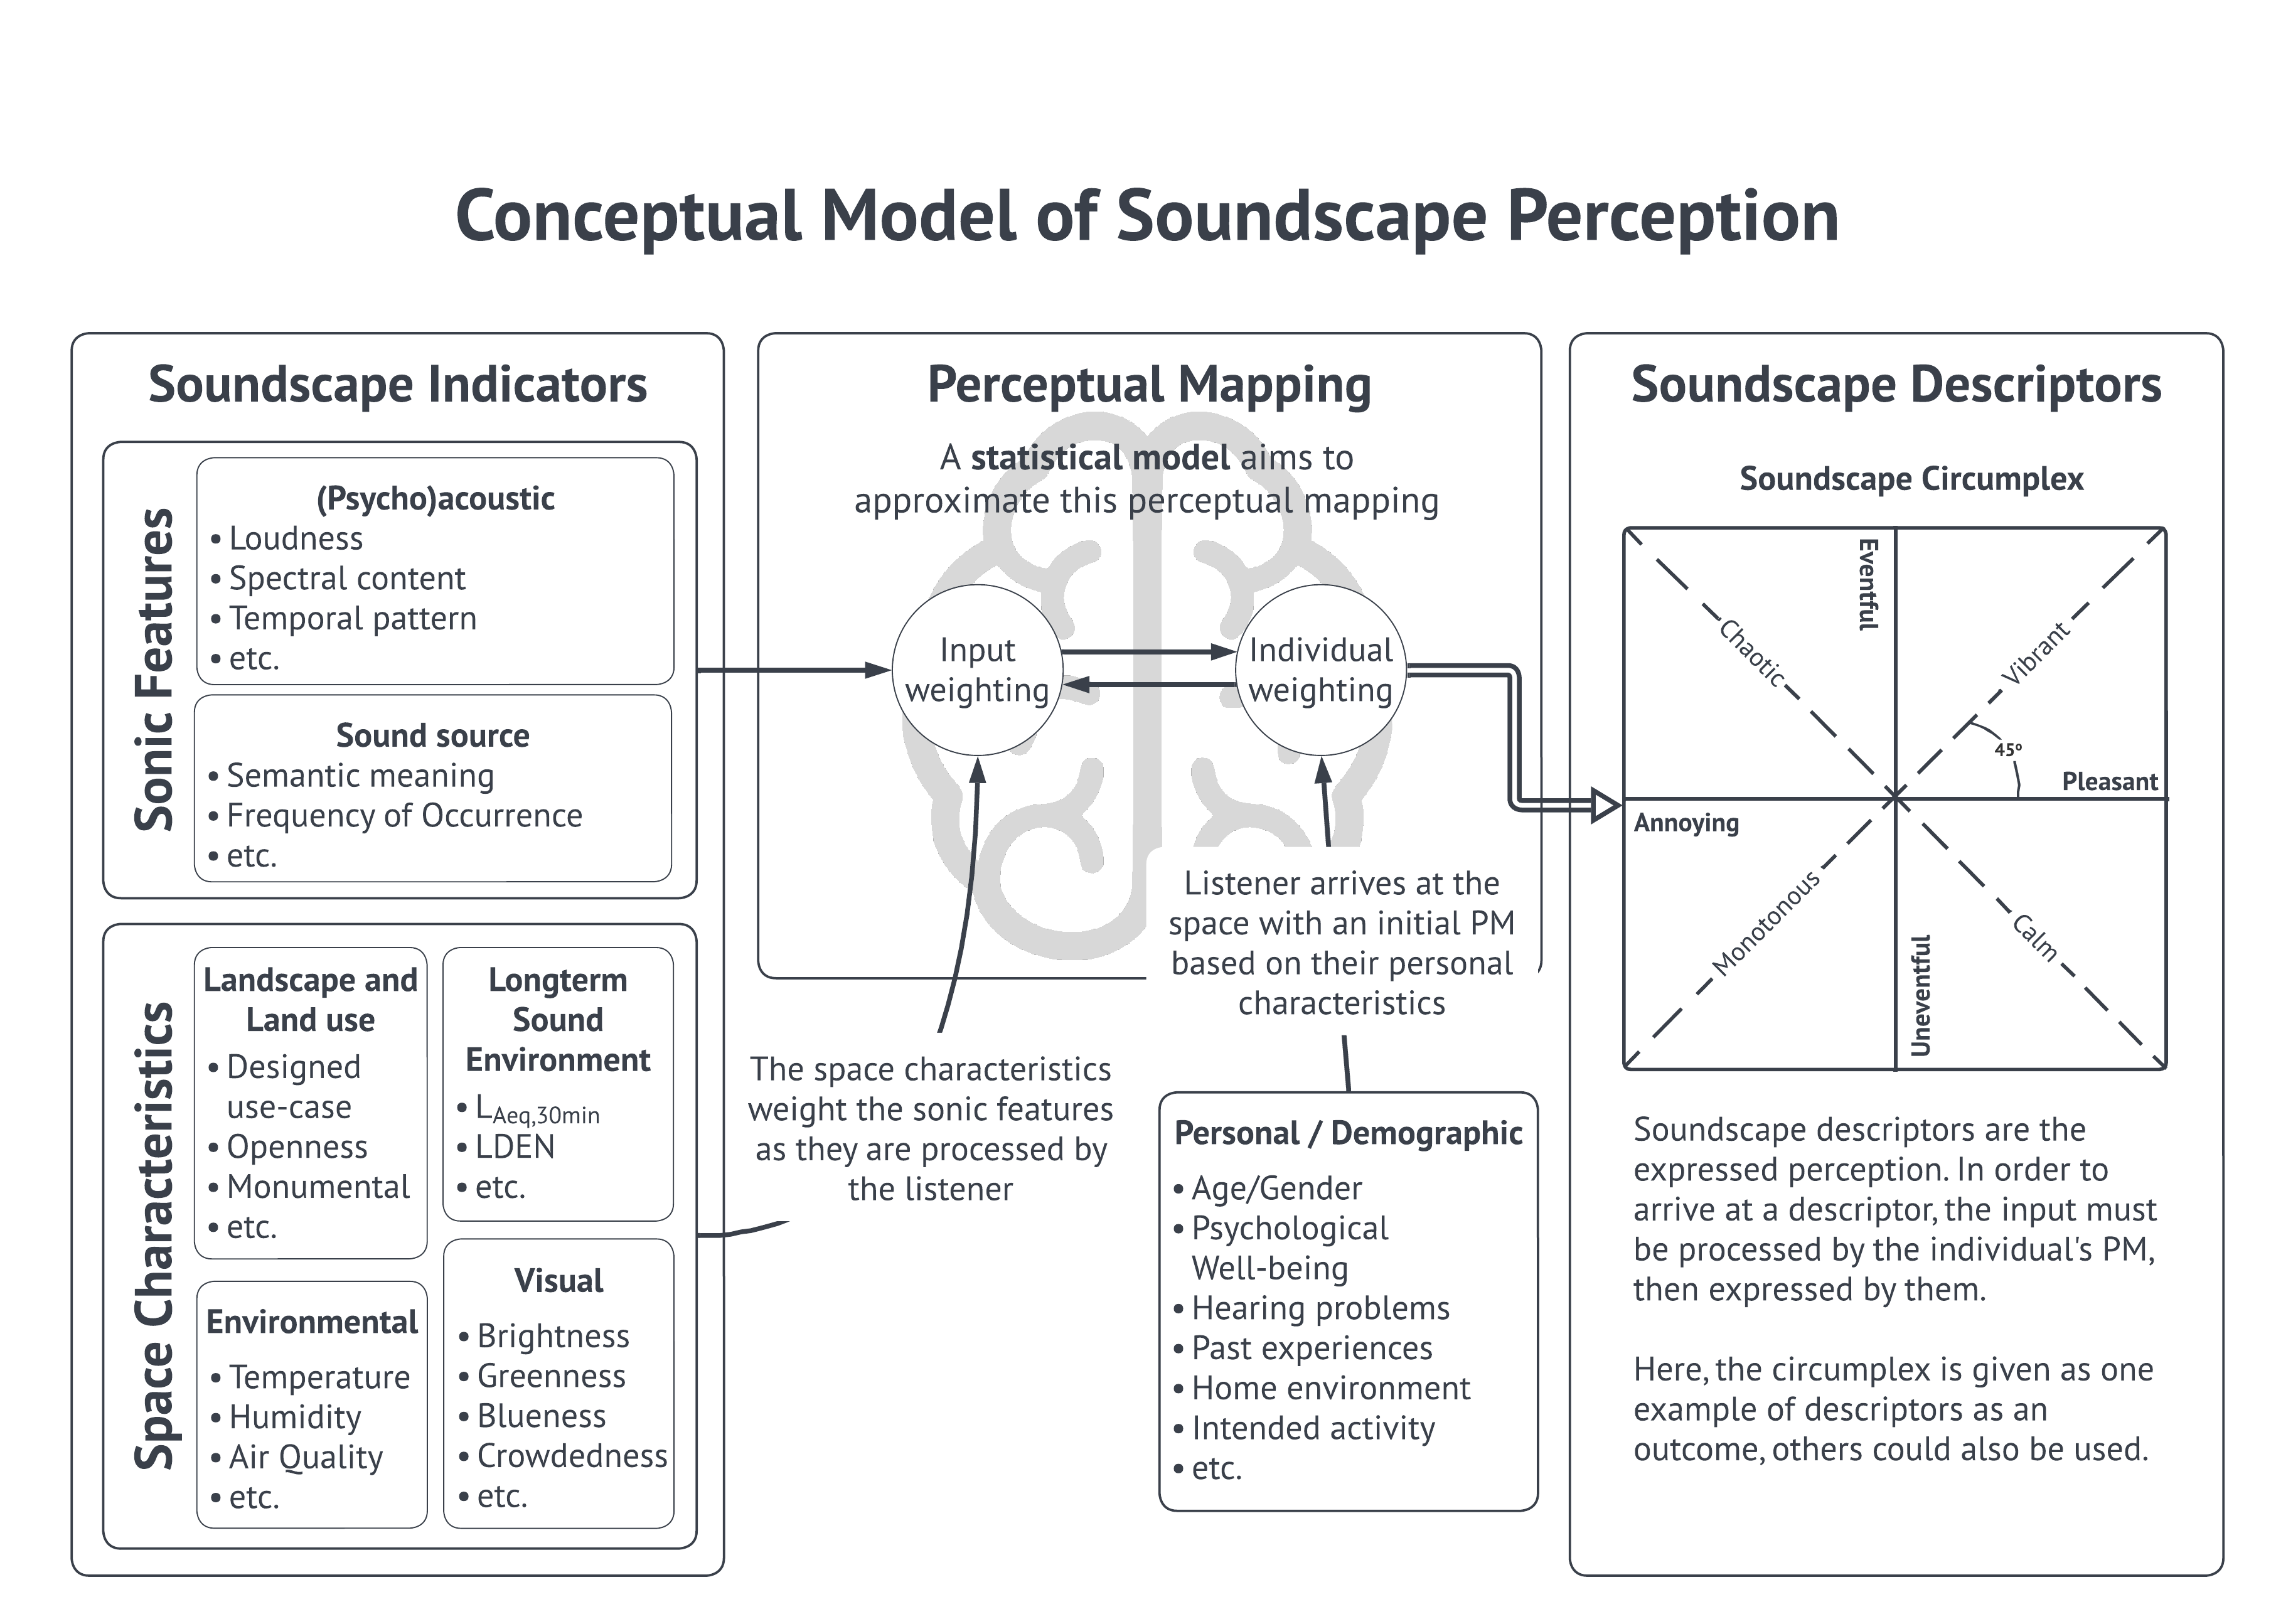
\includegraphics[width=\textwidth]{Figures/Overall Model Concept Diagram_2022-04-28.png}
  \caption{The conceptual model of soundscape perception, illustrating the perceptual mapping from physical inputs, through personal experience, to soundscape descriptors. The role of the statistical model is to attempt to approximate or reflect this perceptual mapping. \label{fig:percepMap}}
\end{figure}

According to a recent review of predictive soundscape models from \citet{Lionello2020systematic}, the degree of employing auditory and non-auditory factors in soundscape prediction varies, with some studies relying on contextual, personal/demographic \citep{Erfanian2021Psychological,Tarlao2020Investigating} or social media \citep{Aiello2016Chatty} data entirely to predict and generate soundscape features. Some methods also incorporate perceptually-derived features, such as subjective sound level and visual pleasantness as predictors \citep{Lionello2020systematic}. In general, these methods which incorporate perceptually-derived inputs achieve better accuracy rates than those which don't, however this information must also be obtained from people via a survey and therefore are unsuitable for predictive modelling where surveys are not possible. For example, \citet{Ricciardi2015Sound} proposed two models based on data collected from a smartphone application to predict urban sound quality indicators based on linear regressions. The first model which incorporated perceptually-derived input features (visual quality and familiarity) achieved an $R^2$ of 0.72, while a second model without these features achieved an $R^2$ of 0.58. This indicates the necessity for considering and accounting for the influence which contextual factors in a space have on the relationship between the sound environment itself and the listener's perception of it (i.e. the soundscape) while also highlighting the challenges associated with a predictive model which depends only on measurable features.

\subsection{Psychoacoustic Models}

\subsubsection*{Zwicker \& Fastl}

\paragraph*{Annoyance}Models for the prediction of annoyance have been previously proposed, with the most notable model based on psychoacoustic metrics proposed by \citet{PsychoacousticsfactsmodelsZwicker}. The authors provide definitions and the empirical basis behind a series of psychoacoustic metrics (loudness, roughness, sharpness, fluctuation strength), the specifics of which will be further expanded upon in \cref{chap:methods}. Briefly, these metrics relate to specific psychophysical sensations which move beyond the strictly physical descriptions of sounds. Acoustical metrics such as \gls{lzeq} describe the physical characteristics of a sound, derived from the magnitude of the pressure changes induced by the sound. By contrast, psychoacoustical metrics attempt to relate these physical characteristics to the sensation they induce in humans. They therefore provide a more direct insight into how sounds are perceived and interpreted by a listener. 

Each of the proposed psychoacoustic metrics therefore attempts to describe one aspect of the sonic quality of the sound such that a sound can be broken down and described through some combination of these metrics. Zwicker and Fastl then propose a model which combines these metrics to quantitatively describe annoyance ratings obtained in psychoacoustic experiments. From \citet[p. 327]{PsychoacousticsfactsmodelsZwicker}:

\begin{quotation}
  Basically, psychoacoustic annoyance depends on the loudness, the tone colour, and the temporal structure of sounds. The following relation between psychoacoustic annoyance, \gls{pa} and the hearing sensations loudness, N, sharpness, S, fluctuation strength, F, and roughness, R can be given:

  \begin{equation}
    \label{eqn:pa1}
    PA \sim N( 1 + \sqrt{[g_1(S)]^2 + [g_2(F, R)]^2})
  \end{equation}

\end{quotation}

Based on the results of psychoacoustic experiments, the authors expand on this theory to provide the following general model of psychoacoustic annoyance:

\begin{equation}
  PA = N_5 ( 1 + \sqrt{w^2_s + w^2_{FR}})
\end{equation}

with 

\begin{itemize}
  \item \gls{n5} percentile loudness in sone
  \item $w_s = (\frac{S}{acum} - 1.75) * 0.25 \log{(\frac{N_5}{sone} + 10)}$ for $S > 1.75$ acum
\end{itemize}

describing the effects of sharpness S and 

\begin{itemize}
  \item $w_{FR} = \frac{2.18}{(N_5/sone)^{0.4}} (0.4 * \frac{F}{vacil} + 0.6 * \frac{R}{asper})$
\end{itemize}

describing the influence of fluctuation strength F and roughness R.

% TODO: Add more here

%TODO: Not a great description here
\paragraph*{Sensory pleasantness} In addition to the more common psychoacoustic annoyance, Zwicker and Fastl also present a mode for what they term `sensory pleasantness'. Like annoyance, pleasantness is influenced by the elementary psychoacoustic sensations of loudness, roughness, sharpness, and tonality. Due to the complexity of the sensation of pleasantness, the model predicts the `relative pleasantess' rather than an absolute metric. Their equation is based on relative values of sharpness, S, roughness, R, tonality T, and loudness N, \citep[p. 245]{PsychoacousticsfactsmodelsZwicker}:

\begin{equation}
  \frac{P}{P_0} = e^{-0.7 R/R_0} e^{-1.08 S/S_0} (1.24 - e^{-2.43 T/T_0} e^{-(0.023 N/N_0)^2})
\end{equation}
%TODO: Add discussion of Zwicker annoyance and sensory pleasantness models

\subsection{Structural Equation Models}

\gls{sem} is a statistical approach to testing hypotheses about relationships between variables and latent features. \gls{sem} is a flexible approach in that it can include one or more independent or dependent variables and the variables can be continuous or discrete, factors or measured. As a collection of statistical methods, \gls{sem} is focussed on causal inference and is fundamentally built on a combination of path diagrams and regression modelling techniques \citep{Ullman2012Structural}. Most frequently in an \gls{sem}, the researcher constructs a path diagram which expresses the hypothesised relationships between the variables of interest. These path diagrams can be quite complex, including covariance relationships, latent variables, residuals, and distinctions between factors and measured variables. The model is then fit to the data through a selected estimation method (most typically Maximum likelihood (ML) as in regression modelling) and evaluated. The model may then be further reduced or modified if necessary. \gls{sem} also allows for multilevel modelling where separate models are developed for different levels of a nested hierarchy. This is conceptually equivalent to the \gls{mlm} or \gls{lmer} discussed throughout this thesis. 

Several studies in the soundscape literature have made use of \gls{sem}. \citet{Tarlao2020Investigating} constructed a \gls{sem} to investigate the influence of contextual and personal factors on soundscape perception.
%TODO: Continue discussion of sem in soundscape.  

\subsection{Models based on non-acoustic data sources}

\citep{Verma2020Predicting}, \citep{Gasco2020Social}

\subsection{Red and Green Soundscape Indices}
\citep{Yang2022Effects,Kogan2018Green} 

\subsection{Clustering/Classification Approach}
%FIXME: Probably needs to go to a new location
%TODO: Review Sun 2019 Classification
One approach which may seem promising is to generate clusters of soundscapes. \draft{Review ref on this -> \citet{Sun2019Classification}}. Soundscape perception of a space has many dimensions and can be difficult to adequately express. Clustering analysis provides a method to investigate the patterns present in a high-dimensional dataset and aid interpretation while imposing minimal starting assumptions. Within soundscape, this would enable the identification of 'soundscape types' based on some combination of perceptual, physical, and architectural data. 

For the purposes of predictive soundscape modelling with the characteristics laid out above, clustering would allow us to identify perceptual types, into which a soundscape could be placed based on its physical features. This process is outlined in \cref{fig:clusterModel}. Once the combined perceptual, contextual, and physical data are collected, unsupervised clustering analysis is performed on the perceptual data, including all \glspl{paq}, the overall questions, and perhaps demographic data. Once the clusters are identified. prior knowledge and information about the architectural typologies and use cases are used to inform the selection of appropriate descriptive labels for the clusters. Then... %TODO: Continue clustering discussion.

\begin{figure}
  %TODO: Create clustering approach model
  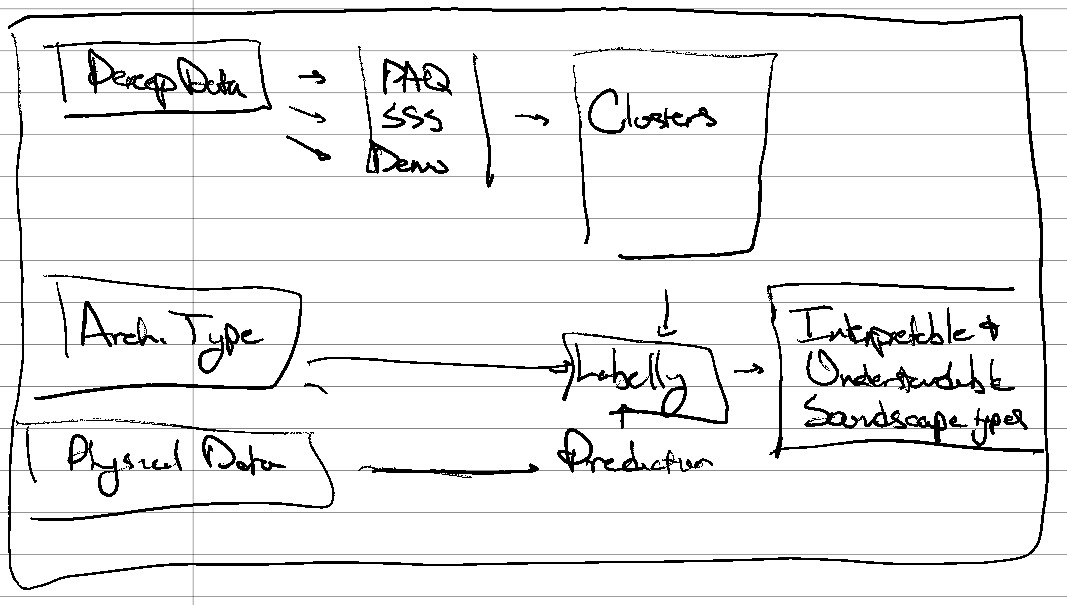
\includegraphics[width=\textwidth]{Figures/Remarkable clustering figure.jpg}
  \caption{Draft figure of a clustering approach}\label{fig:clusterModel}
\end{figure}

\draft{Issue with this approach to expand on: Limitations of starting dataset - impossible to know if we've identified all possible classes. Highly dependent on the primary dataset, the identified clusters cannot extend beyond what was already present.}